\documentclass[thesis2.tex]{subfiles}

\begin{document}
\iffulldocument\else
	\chapter{Conclusions}
\fi

In this thesis, we have explored multi-pulse solutions in three different Hamiltonian systems, two continuous and one discrete. The overarching theme is that multi-pulses only exist with specific geometries, and the spectral stability of multi-pulses is determined by this geometry. Conclusions and suggestions for future exploration specific to each system are given below.

\section{Chen-McKenna suspension bridge equation}

For Chen-McKenna, we are able to fully characterize the spectrum of multi-pulse solutions as long as the individual pulses are well-separated. Using the Krein matrix, we can locate the $n-1$ pairs of interaction eigenvalues associated with an $n$-pulse, and using the Hamiltonian-Krein Index, we can conclude that there are no other potentially unstable eigenvalues. For the multi-pulses with purely imaginary eigenvalues, the next step would be to study their linear and nonlinear stability. Recent work by Nagatou, Plum, and McKenna \cite{Nagatou2019} suggests that only the primary pulse solution may be orbitally stable. The bottom left panel in \cite[Figure 2]{Nagatou2019} corresponds to the first double pulse with purely imaginary interaction eigenvalues. Although they were unable to prove either stability or instability for this case, they have numerical evidence using time-stepping with finite difference methods that the solution is unstable. 

\section{DNLS equation}

For DNLS, we are able to locate the interaction eigenvalues associated with multi-pulses and have extended results which previously only held near the anti-continuum limit to larger values of the coupling constant $d$. We have formulas for the leading order terms of these eigenvalues which are very accurate for intermediate values of the coupling constant $d$. There are several interesting questions which are unanswered. 

Recent work~\cite{Jason2019} has investigated stationary, spatially localized patterns in lattice dynamical systems which change as a parameter is varied (the coupling parameter in this case is fixed). For DNLS, we find a  complex bifurcation structure which arises as the coupling parameter $d$ is varied. In \cref{fig:DNLSbd1f}, we see that if we start with a double on-site soliton and increase $d$ from the anti-continuum limit using AUTO, we reach a turning point. At that point, $d$ starts decreasing, and the solution becomes a double inter-site soliton. Very near the turning point there is a also a bifurcation point; following the solution branch from that bifurcation point, we obtain a solution composed of one on-site soliton and one inter-site soliton. 
\begin{figure}
\begin{center}
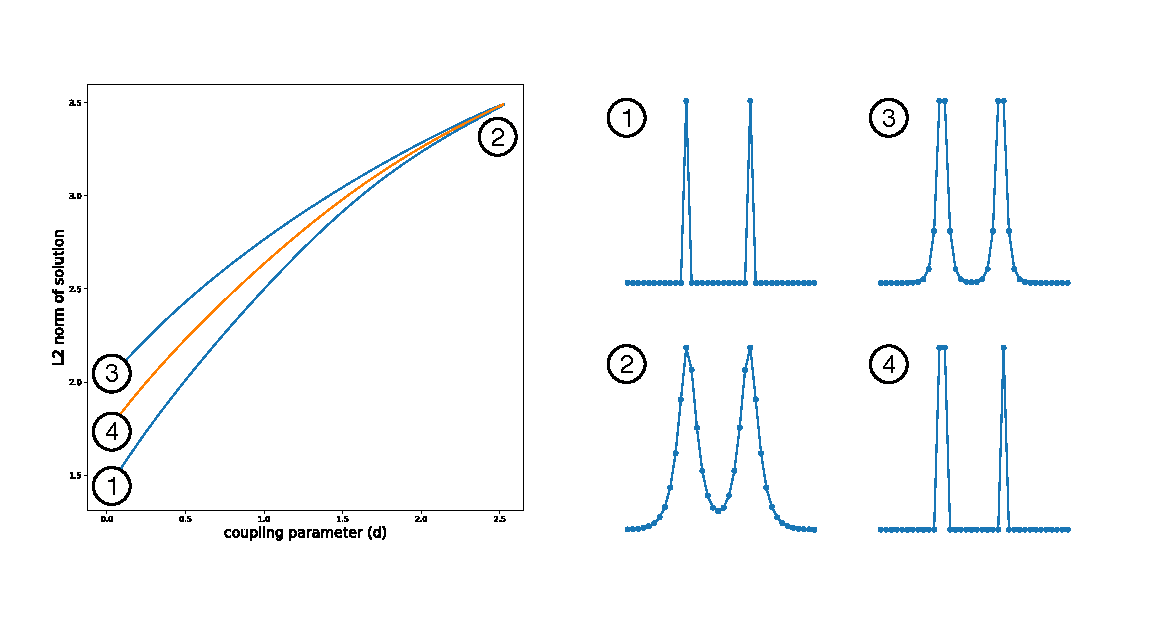
\includegraphics[width=14cm]{images/dnls/bd1.eps}
\end{center}
\caption[Bifurcation diagram in DNLS for increasing $d$]{Bifurcation diagram as $d$ is increased from the anti-continuum limit, starting with double on-site solution. Parameter continuation performed with AUTO.}
\label{fig:DNLSbd1}
\end{figure}
If we continue the parameter continuation using AUTO, we obtain the complex bifurcation structure shown in the left panel of \cref{fig:DNLSbd2}. The right panel of \cref{fig:DNLSbd2} shows the main branch of the bifurcation diagram, which has the form of an isola. This isola passes back and forth between the focusing ($d > 0$) and defocusing ($d < 0$) regimes.
\begin{figure}
\begin{center}
\begin{tabular}{cc}
\includegraphics[width=8cm]{images/dnls/bd2.pdf}
\includegraphics[width=8cm]{images/dnls/bd3.pdf}
\end{tabular}
\end{center}
\caption[Bifurcation diagram in DNLS for increasing $d$]{Bifurcation diagram as $d$ is increased from the anti-continuum limit, starting with double on-site solution. Parameter continuation performed with AUTO.}
\label{fig:DNLSbd2}
\end{figure}

A final avenue of exploration concerns the Ablowitz-Ladik variant of the DNLS equation (AL-DNLS), which can be written as
\begin{equation*}
i\dot{\psi}_n + d(\psi_{n+1} - 2 \psi_n + \psi_{n-1}) + |\psi_n|^2 (\psi_{n+1} + \psi_{n-1}) = 0
\end{equation*}
Unlike DNLS, AL-DNLS has a conserved momentum, which implies that soliton solutions can be centered anywhere in the lattice \cite{Kevrekidis2009}. The linearization about a soliton solution in AL-DNLS has a two-dimensional kernel, as opposed to the one-dimensional kernel for DNLS, which further complicates the analysis. \cite[Figure 5]{Kevrekidis2002} shows two double pulses with the same phase difference of $\pi$ but with different pulse distances; in addition they are on lattices of different sizes. One is spectrally stable and the other is spectrally unstable, which is in direct contrast to what we found for DNLS. It would be interesting to explore what multi-pulses exist for AL-DNLS, and what drives their spectral stability or instability.


\iffulldocument\else
	\bibliographystyle{amsalpha}
	\bibliography{thesis2.bib}
\fi

\end{document}